\documentclass[a4paper,12pt]{article}
\parindent 0pt
\parskip 1mm
\usepackage{amsmath}
\usepackage[dvips]{epsfig}

\begin{document}

\begin{center}

{\Large\bf CN 510 - Principles and Methods of Cognitive and Neural Modeling}

\bigskip

{\large\bf Assignment \# 6}
\smallskip

{\large\bf John Joseph}
\end{center}

\bigskip
{\bf Communcation in Spiking Networks}
\bigskip

This week we are generating an artificial network of spiking neurons and determining their combined effects upon a single post-synaptic neuron. We create the spiking neurons by generating a Poisson spike train which results in a network of neurons with similar ``properties'' (as in mean firing rate) but different spike times throughout our simulation.

\bigskip
{\bf Poisson Input}
\bigskip

The spiking network was simulated by generating a Poisson spike train. As I do not have Matlab, I generated the spike train in C using a formula I found on Wikpedia: Given a uniform distribution between 0 and 1, we randomly select a value from this distribution $U$ and calculate

\begin{equation}
T = \frac{-ln U}{\lambda}
\end{equation}

Where $\lambda$ is our mean spiking rate of 5 Hz. By randomly selecting 60 values we can generate spike timings that should span a mean value of 12 seconds; 5 Hz means 5 spikes/second, so it should take 12 seconds to generate 60 spikes. 

\vspace{2mm}

I chose to model this network on a grid of resolution 1ms, and did this by calculating the spike time as above and casting it as an integer value. This generalyl resulted in a rounding down of my timings, but given the random nature of the distribution I figured that wouldn't matter. 

\vspace{2mm}

The result of this truncation is that we can plot each neuron in our network on a grid, which allows us to definitively determine moments at which neurons fire together. 

\bigskip
{\bf Rotter-Diesmann Synaptic Traces}
\bigskip

The network of 100 neurons was propogated through time using the Rotter-Diesmann integration method. Some consideration was taken to ensure calculations were only carried out during the moment spikes would occur; this was done as follows:

\vspace{2mm}

We pre-calculate our 60 spike times. Then, starting at t=0, we jump to each spike-time and ensure it is properly recorded by taking a look at the values directly preceding it. We then generate the spike, which results in a change in our integration formula that adds a constant term to our exponential propogator. This term, 

\begin{equation}
(B-Cx_i)\delta_i(s(t+1))
\end{equation}

Has a binary value denoted by the $\delta$ that is either a 1 or 0 depending on the presence of a spike. This is what actually generates our sudden increase, and following the spike we allow 10$\tau$ time steps for it to decay back to zero before continuing to the next spike (where $\tau$ is our time constant).

\vspace{2mm}

Special care must be taken to determine whether or not another spike will occur duing this decay period; this was done in C as follows:

\begin{verbatim}
decay = (interval < tau*10) ? currentTime+interval : currentTime+tau*10;
\end{verbatim}

Where decay is how much time we allow it to decay, currentTime is our current time, and interval is the time until our next spike. 

\vspace{2mm}

The assignment asked us to plot our network of 100 neurons for three values of $C$: 0,1,and 0.5. $C$ serves as an inhibitory term, and often did well to keep our spikes in check. As you will see, the case where $C=0$ resulted in spike values greater than 1; this is because of the addition that results when spikes occur mid-decay. This was largely kept in check when $C$ was 1, where during these events the spike values seemed to be capped at 1. 

\vspace{2mm}

The plots below show neurons 86 in blue and 28 in red; this was a completely random choice, as were the spike trains. With that said, the random Poisson trains were impossible to keep consistent. 

\vspace{2mm}

The first plot below shows the rastergram, which depicts the presence of a spike for each neuron at each time step (~12000). 

\vspace{2mm}

The remaining three plots show each value of C; note the relatively large spike values observed in the $C=0$ plot.

\vfil\eject
 \begin{center}
\begin{figure}[h!]
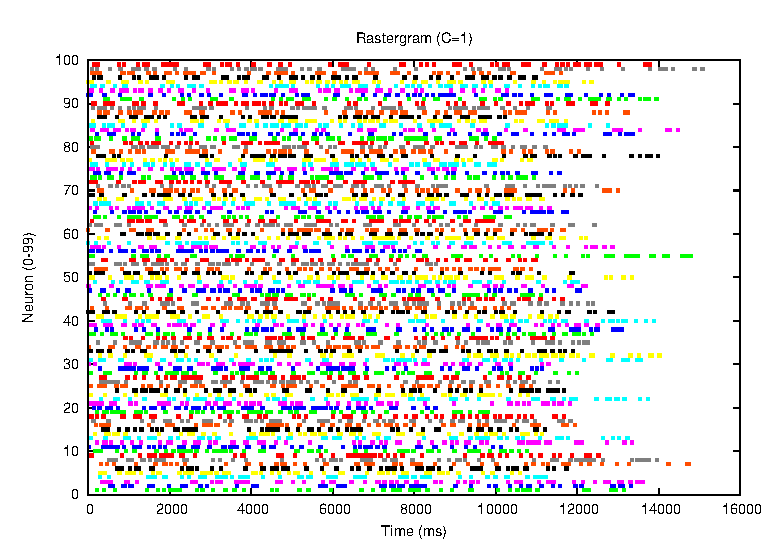
\epsfig{file=data/figures/raster1,width=15cm,height=8cm}
\caption{\label{pict1}Rastergram of all neurons (I hope it's not too jumbled)}
\end{figure}

\begin{figure}[h!]
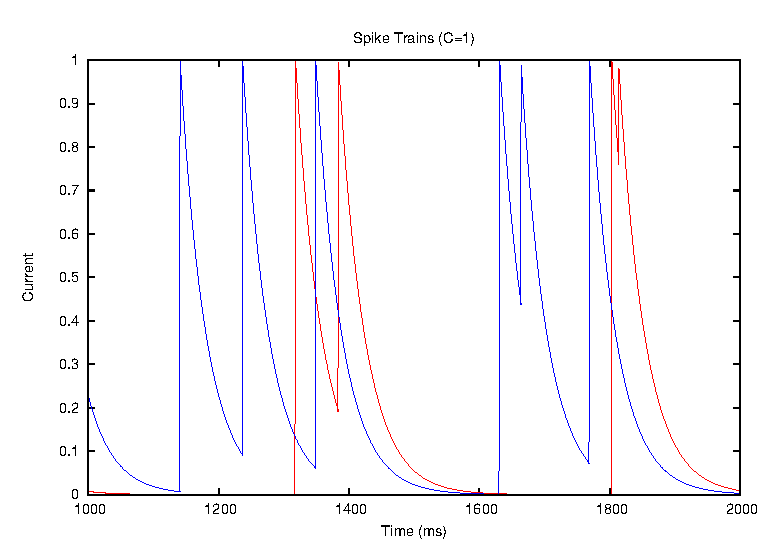
\epsfig{file=data/figures/zoom1,width=15cm,height=8cm}
\caption{\label{pict1}C=1 for neurons 86(red) and 28(blue)}
\end{figure}

\begin{figure}[h!]
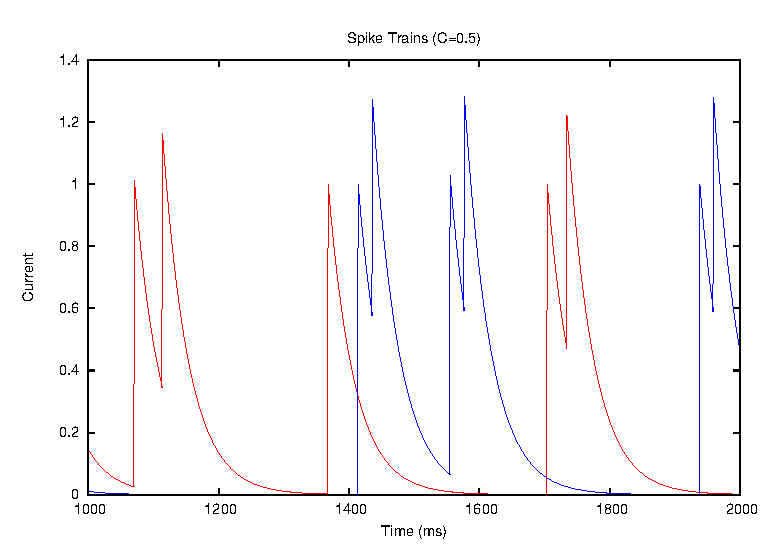
\epsfig{file=data/figures/zoom05,width=15cm,height=8.5cm}
\caption{\label{pict1}C=0.5 for neurons 86(red) and 28(blue)}
\end{figure}

\begin{figure}[h!]
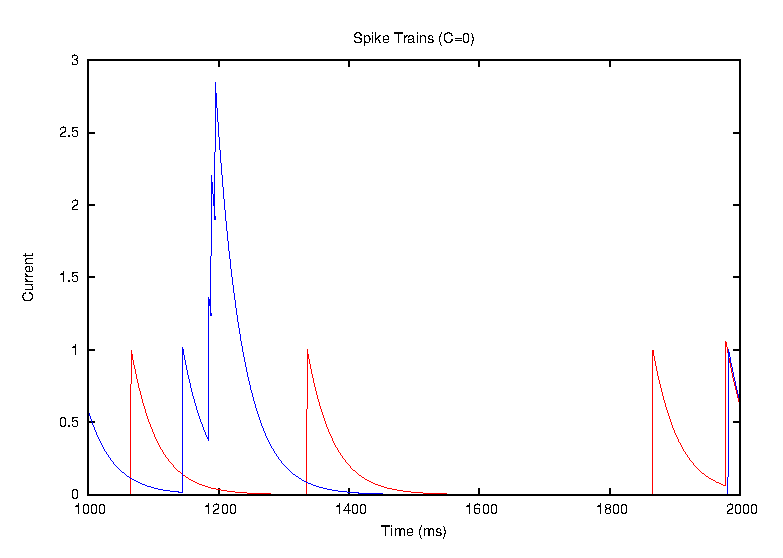
\epsfig{file=data/figures/zoom0,width=15cm,height=8.5cm}
\caption{\label{pict1}C=0 for neurons 86(red) and 28(blue)}
\end{figure}
\end{center}

\vfil\eject

After plotting these three values, we were asked to change our spiking term as follows

\begin{equation}
(B-0.01Cx_i)\delta_i(s(t+1))
\end{equation}

I wasn't sure if we were asked to plot this function separately for two neurons as before, but the results were what you'd expect. The multiplier on C made it nearly negligible, resulting in a case similar to our $C=0$ situation before, and spikes regularly achieved values higher than 1. Excluded from the report is the case where C=0 did not matter here, since the multiplier went to zero regardless.
\begin{center}
\begin{figure}[h!]
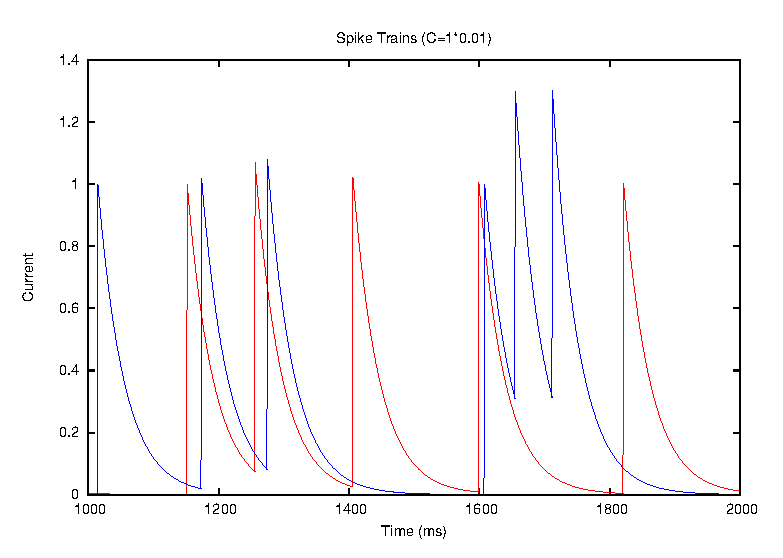
\epsfig{file=data/figures/zoomM_1,width=15cm,height=10cm}
\caption{\label{pict1}C=1x0.01 for nuerons 86 (red) and 28 (blue)}
\end{figure}

\begin{figure}[h!]
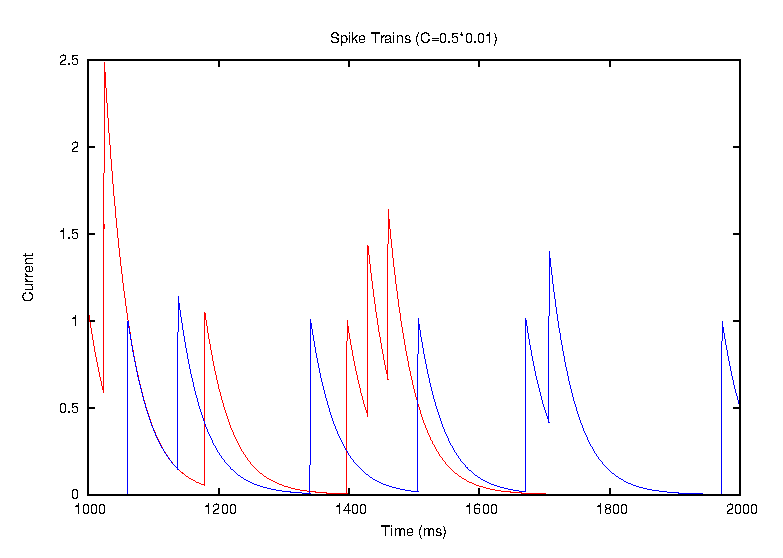
\epsfig{file=data/figures/zoomM_05,width=15cm,height=10cm}
\caption{\label{pict1}C=0.01x0.5 for neurons 86 (red) and 28 (blue)}
\end{figure}
\end{center}

\vfil\eject


Though it will be further discussed in the next section, we were also asked to determine the cumulative current for out network; that is, determine the sum of all neuronal currents at each time step. The effects of this multiplier (0.01) onthe cumulative sum was what I would call negligible. The degree of randomness in our data generation made it hard to tell (perhaps I should have generated one spike train at the beginning and stuck with it), but the values between 1000ms and 2000ms seemed to range between similar values with or without the 0.01.  

\vspace{2mm}

The top graph shows the case where $C=0$, and the multiplier does not matter. For the bottom two, the multiplier case is on the right. The values do actually peak at slightly higher values, which is what we'd expect given a lower inhibtory term. I can see how this lowering would be useful, particularly in the case where repeated stimulus is something to look out for but inhibition was still required. 

\vspace{2mm}

That being said, in our random spike train example I really didn't see the point in inducing such a small change on our system. 

\vfil\eject

\begin{figure}[h!]
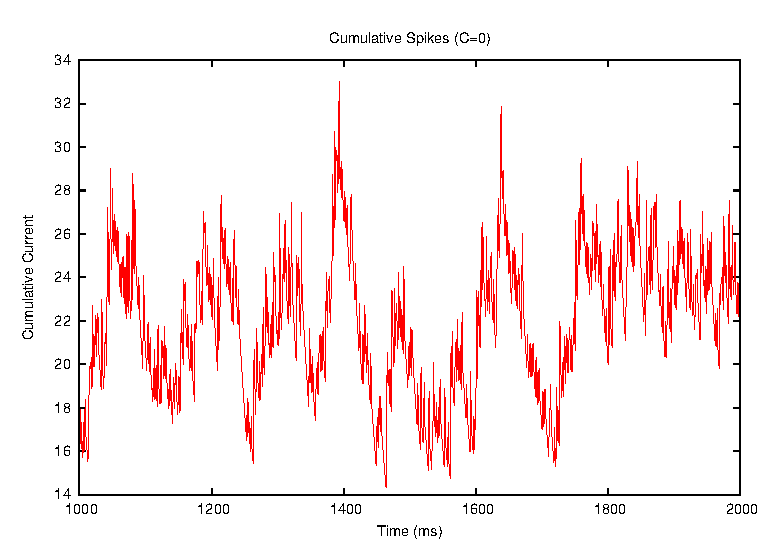
\epsfig{file=data/figures/xCum0,width=15cm,height=12cm}
\caption{\label{pict1}Cumulative Currents for C=0}
\end{figure}

\begin{figure}[h!]
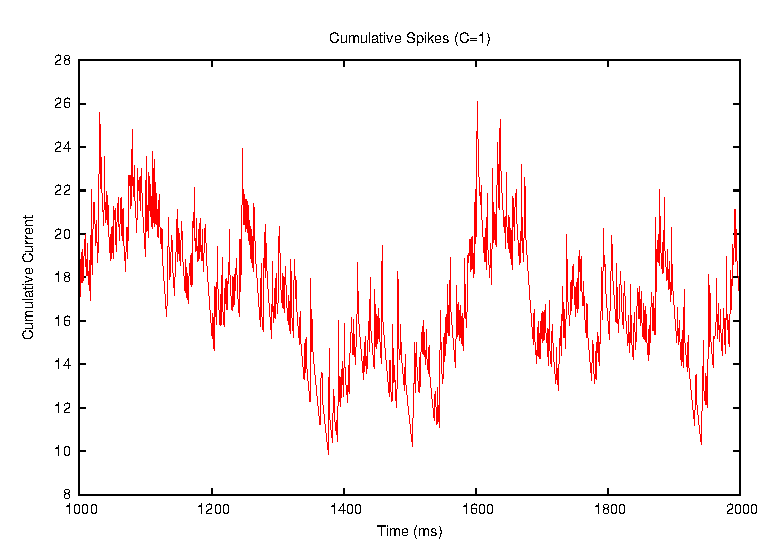
\epsfig{file=data/figures/xCum1,width=8cm,height=6cm}
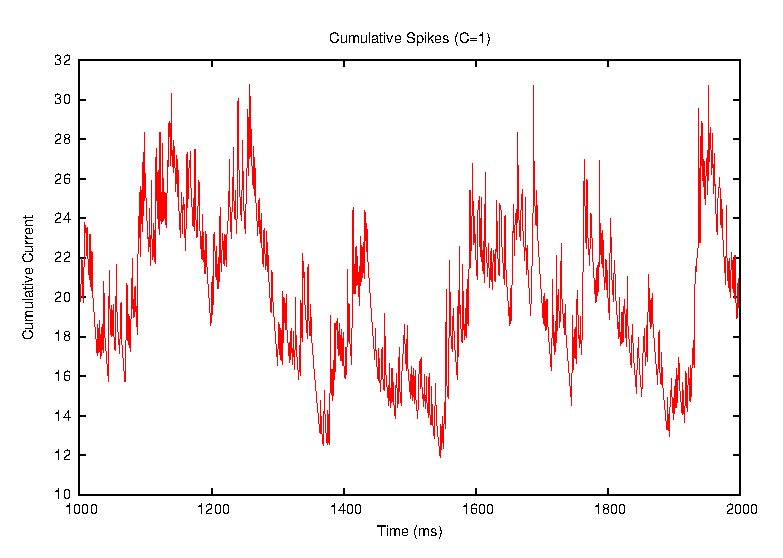
\epsfig{file=data/figures/xCumM_1,width=8cm,height=6cm}
\caption{\label{pict1}Cumulative Currents for C=1 and C=0.01x1}
\end{figure}

\begin{figure}[h!]
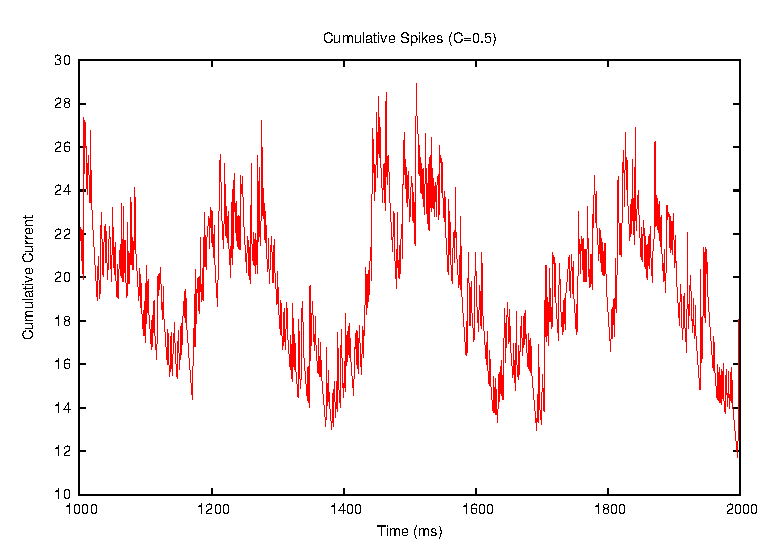
\epsfig{file=data/figures/xCum05,width=8cm,height=6cm}
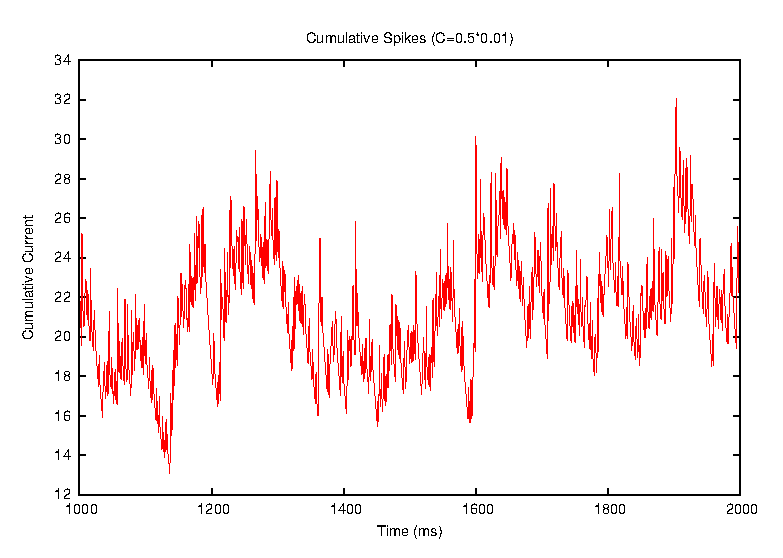
\epsfig{file=data/figures/xCumM_5,width=8cm,height=6cm}
\caption{\label{pict1}Cumulative Currents for C=0.5 and C=0.01x0.5}
\end{figure}

\vfil\eject

\bigskip
{\bf Rotter-Diesmann Postsynaptic Cell}
\bigskip
In addition to simulating this network, we were asked to funnel the network's output into a single neuron and determine the post-synaptic effects. These effects depend on the cumulative spiking values. Thes values are found by summing the current of our entire network at each time step. 

\vspace{2mm}

We are asked to discuss the strengths and weaknesses of different C values on the integrating properties of this post-synaptic neuron. Taking a look at my plots, we can see that the post-synaptic neuron did not do too badly as an integrator. In my opinion it looks as though the higher C values like 1 and 0.5 did a better job than when $C=0$, although we are looking at a small slice of the overall behavior.

\vspace{2mm}

I couldn't really give a reason for this, as the previous plots the $C=0$ case was more erratic, but its cumulative plot appears to be the most ``muted'' of the three. This is the opposite of what I expected, as I had thought the varying values of that plot would more accurately contribute to the cumulative voltage function. 
\begin{center}

\begin{figure}[h!]
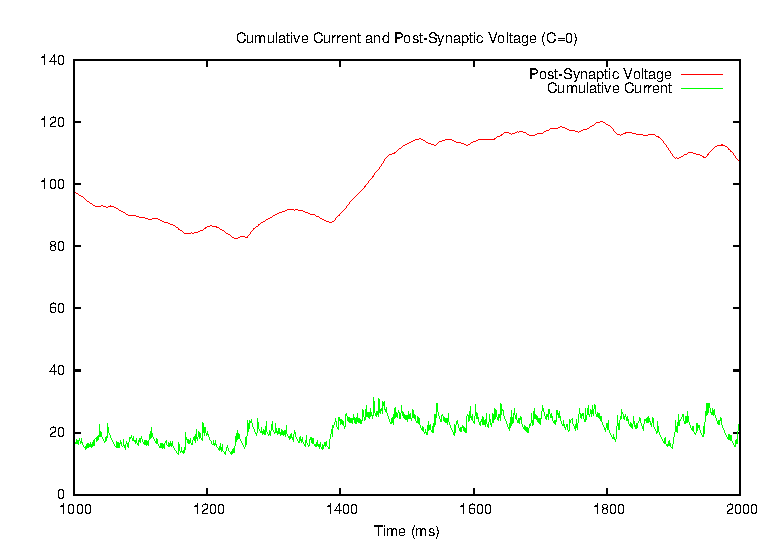
\epsfig{file=data/figures/partB_0,width=15cm,height=7cm}
\caption{\label{pict1}Post-Synaptic Voltage and Cumulative Current, C=0}
\end{figure}

\begin{figure}[h!]
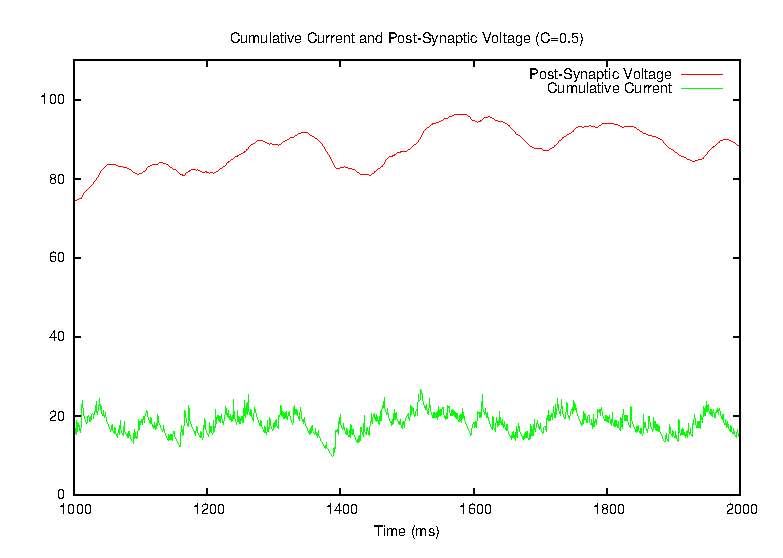
\epsfig{file=data/figures/partB_05,width=15cm,height=7cm}
\caption{\label{pict1}Post-Synaptic Voltage and Cumulative Current, C=0.5}
\end{figure}


\begin{figure}[h!]
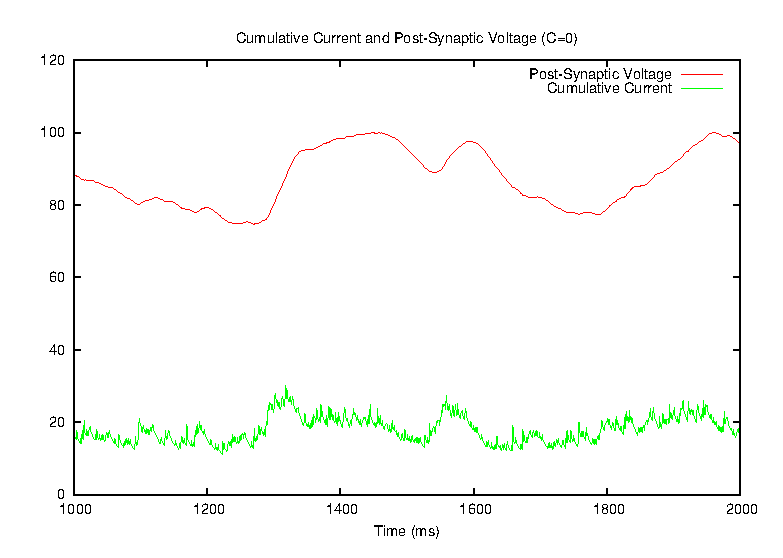
\epsfig{file=data/figures/partB_1,width=15cm,height=7cm}
\caption{\label{pict1}Post-Synaptic Voltage and Cumulative Current, C=1}
\end{figure}
\end{center}
\vfil\eject

\bigskip
\bigskip
\bigskip
\vspace{10mm}
{\bf Extra Credit}
\bigskip

The extra credit asked us to simulate a synapse using the alpha function as outlined in the Rotter Diesmann paper. I did this in C as follows:
\vspace{15mm}
\begin{verbatim}
double DT = 0.02;
double y=0, dy=1;
double t=0;
double A=50,B=50;
      
while (t<1)
  {
     if (A==B)
     {//alpha
        dy=exp(-A*DT)*(dy+B*y);
        y=(DT*exp(-A*DT))*(dy+B*y)+y*exp(-A*DT);
     }
     else
     {//beta
        dy=exp(-A*DT)*(dy+B*y);
        y=(1/(B-A))*(exp(-A*DT)-exp(-B*DT))*(dy+B*y)+y*exp(-B*DT); 
     }
     t+=DT;
  }
\end{verbatim}

My idea was to carry out the matrix multiplication outlined in the paper by hand and then implement the resulting formula. The results however, must be incorrect as the simulation is very unstable for values of A or B lower than the ones I've used. I don't know why this is, and if I plot the analytic solution as a function of t it behaves as expected. 

\vspace{2mm}

The time constant is technically correct at $A=50$, I think, but the values here are very very low. Also, I was rather disappointed that I couldn't replicate the plot in the paper. As such I don't really feel as though I deserve the extra credit, but I figured I may as well include the plot and code. 

\begin{figure}[h!]
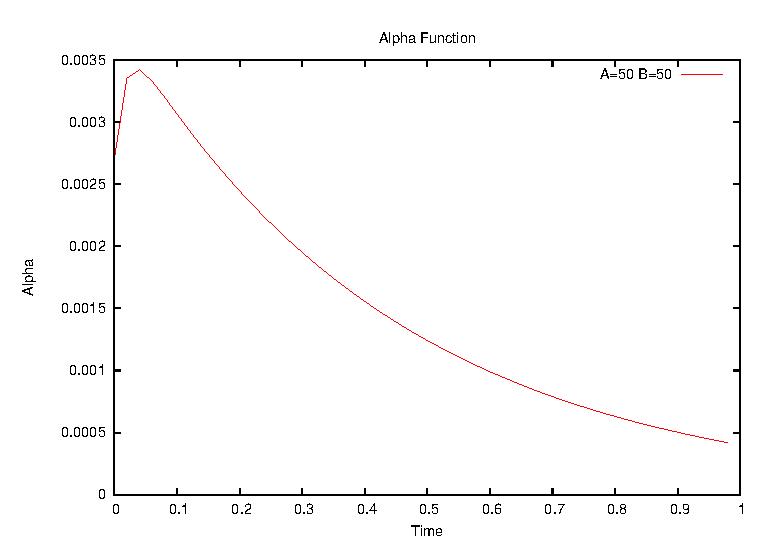
\epsfig{file=data/figures/alpha,width=15cm,height=12cm}
\caption{\label{pict1}Alpha Function as outlined above}
\end{figure}

\end{document}
